% ============================================
\section{Przegląd modułów}
% ============================================

\subsection{Moduł I --- Podstawowe dane}

\begin{frame}[t]{Moduł I}{Podstawowe dane}
  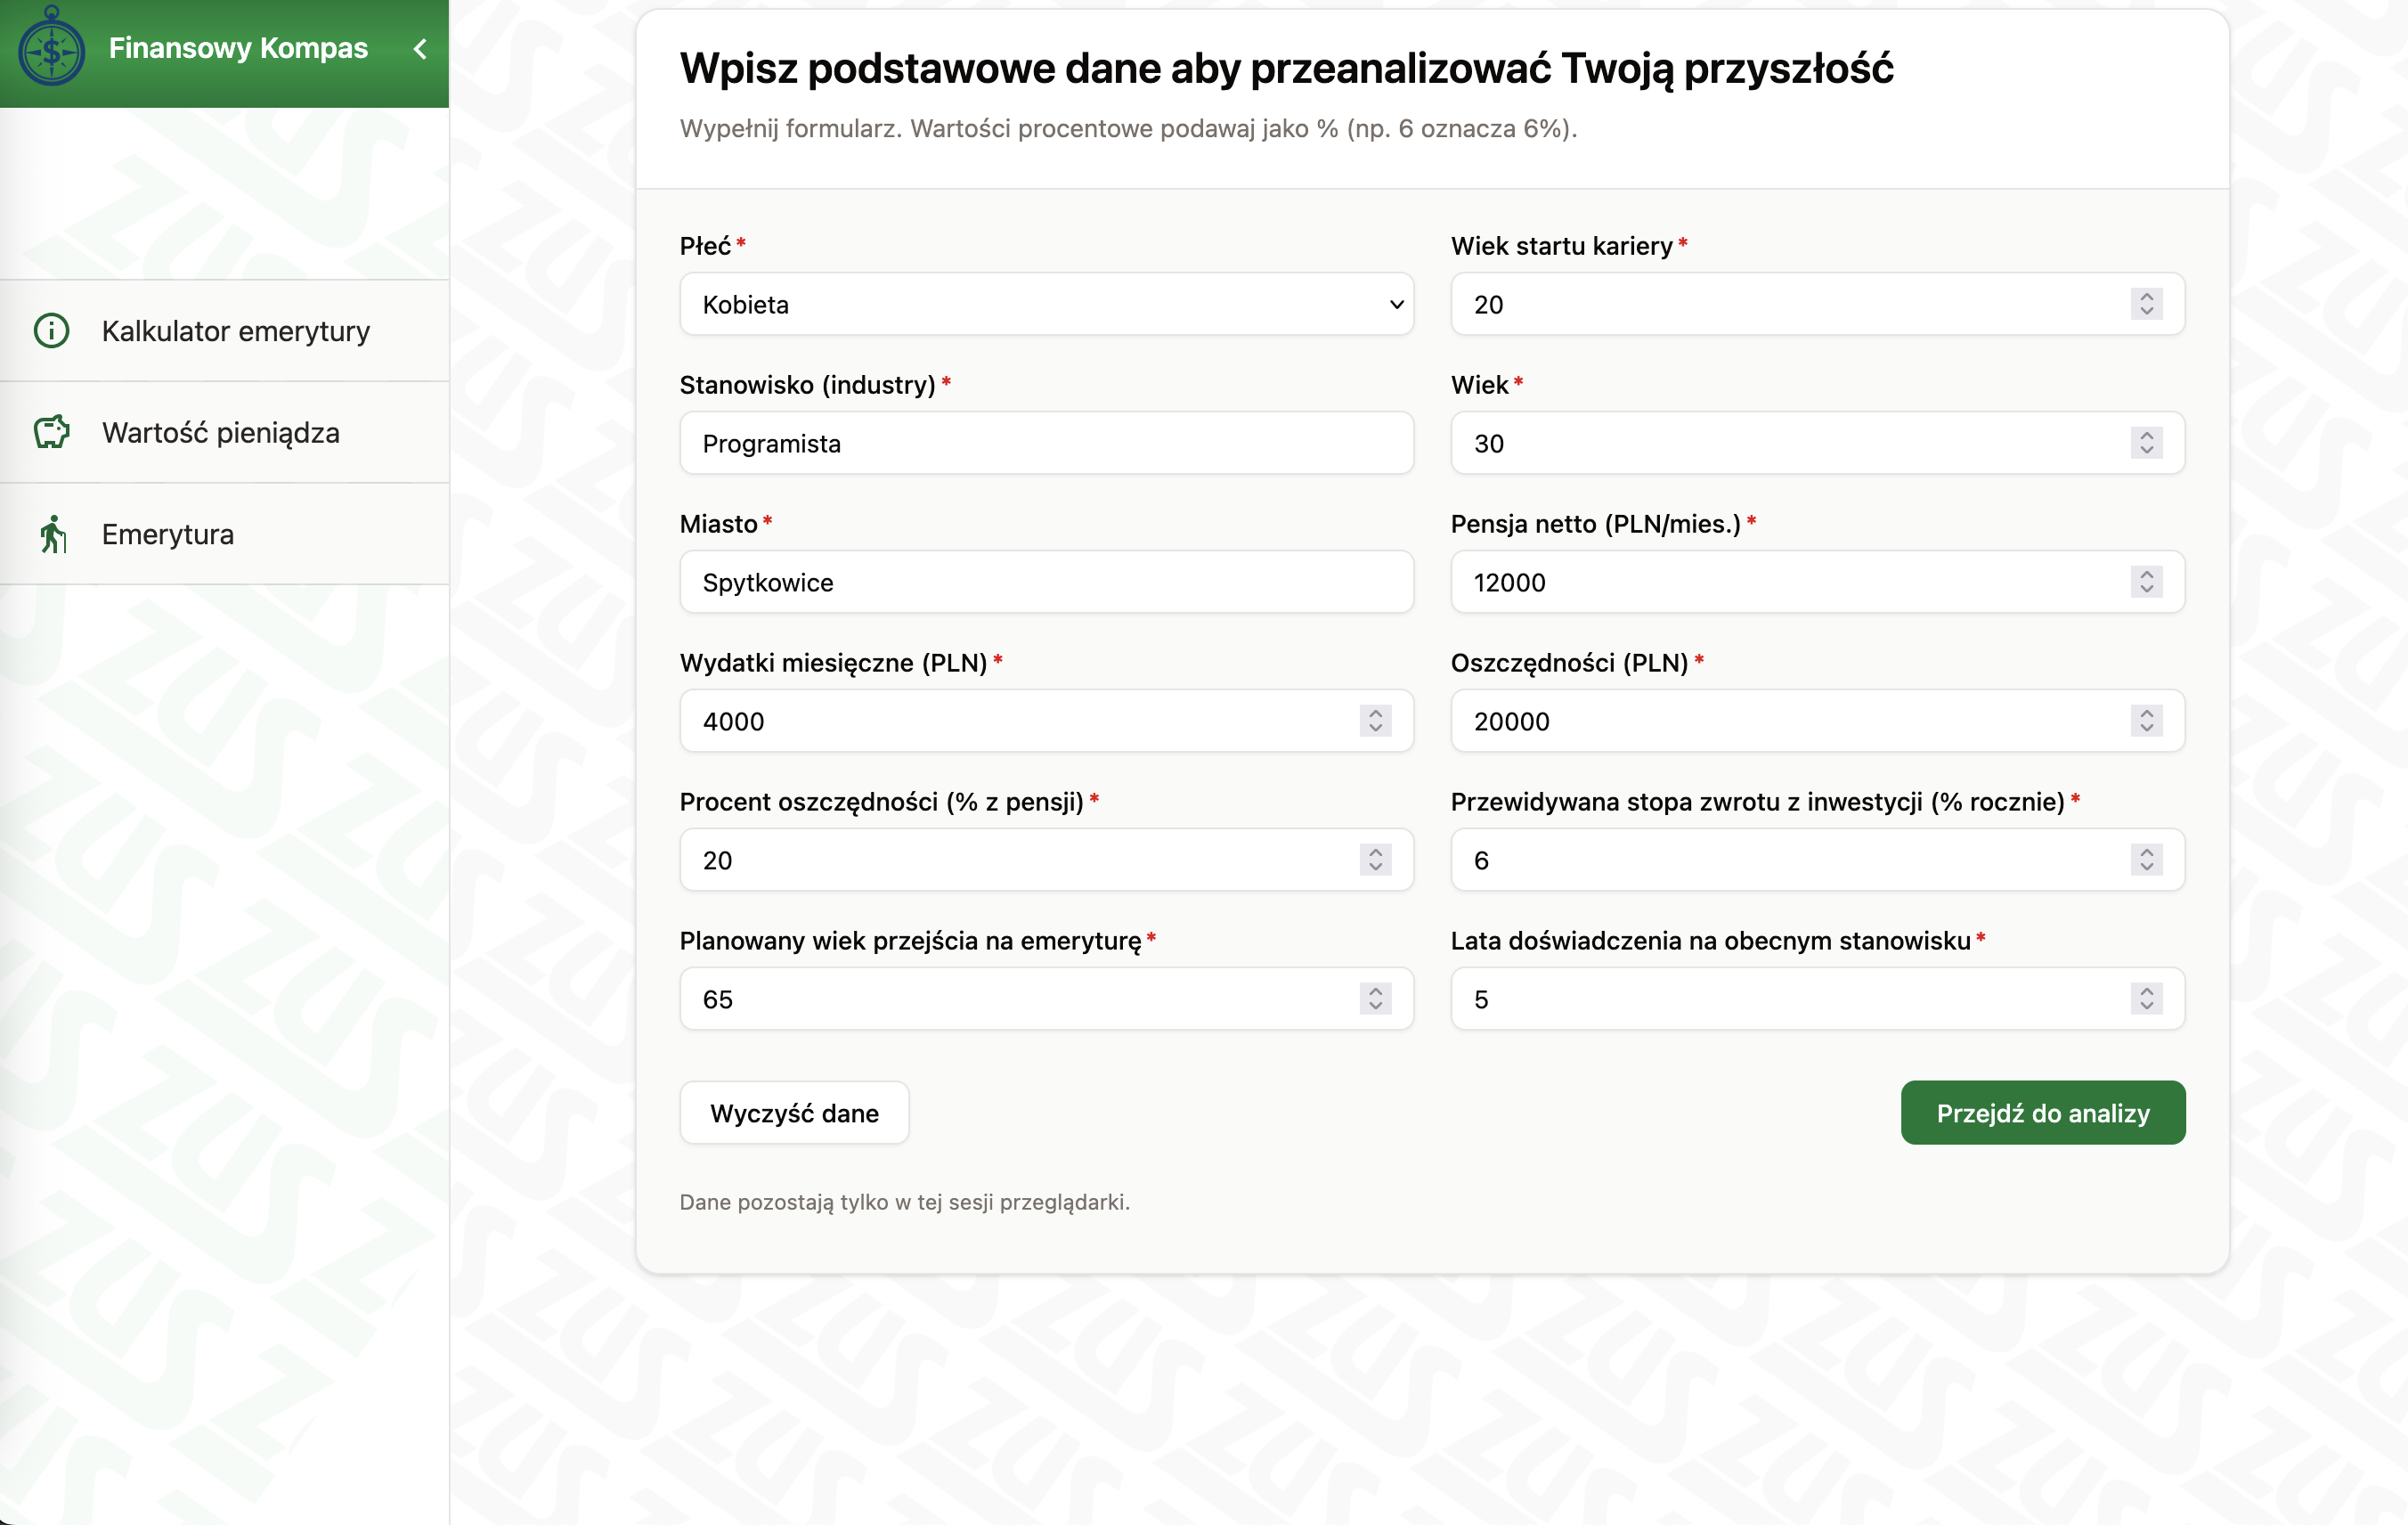
\includegraphics[width=.8\textwidth]{img/module_1_basic_data}
\end{frame}

\begin{frame}[t]{Moduł I}{Podstawowe dane}
Przy minimalnym zestawie danych przekazanych przez użytkownika:
\pause
\begin{itemize}
  \item zawód/branża,
  \pause
  \item miejscowość zamieszkania,
  \pause
  \item wiek,
\end{itemize}
\pause
nasz system od razu wylicza wstępny model finansowy:
\begin{itemize}
  \pause
  \item projekcję wynagrodzeń (w ujęciu nominalnym i realnym),
  \pause
  \item miesięczne wydatki i oszczędności, lata doświadczenia, wiek przejścia na emeryturę —
        wszystkie wartości można w każdej chwili doprecyzować ręcznie.
\end{itemize}
\end{frame}

\subsection{Moduł II --- Uproszczony kalkulator emerytalny}

\begin{frame}[t]{Moduł II}{Uproszczony kalkulator emerytalny}
  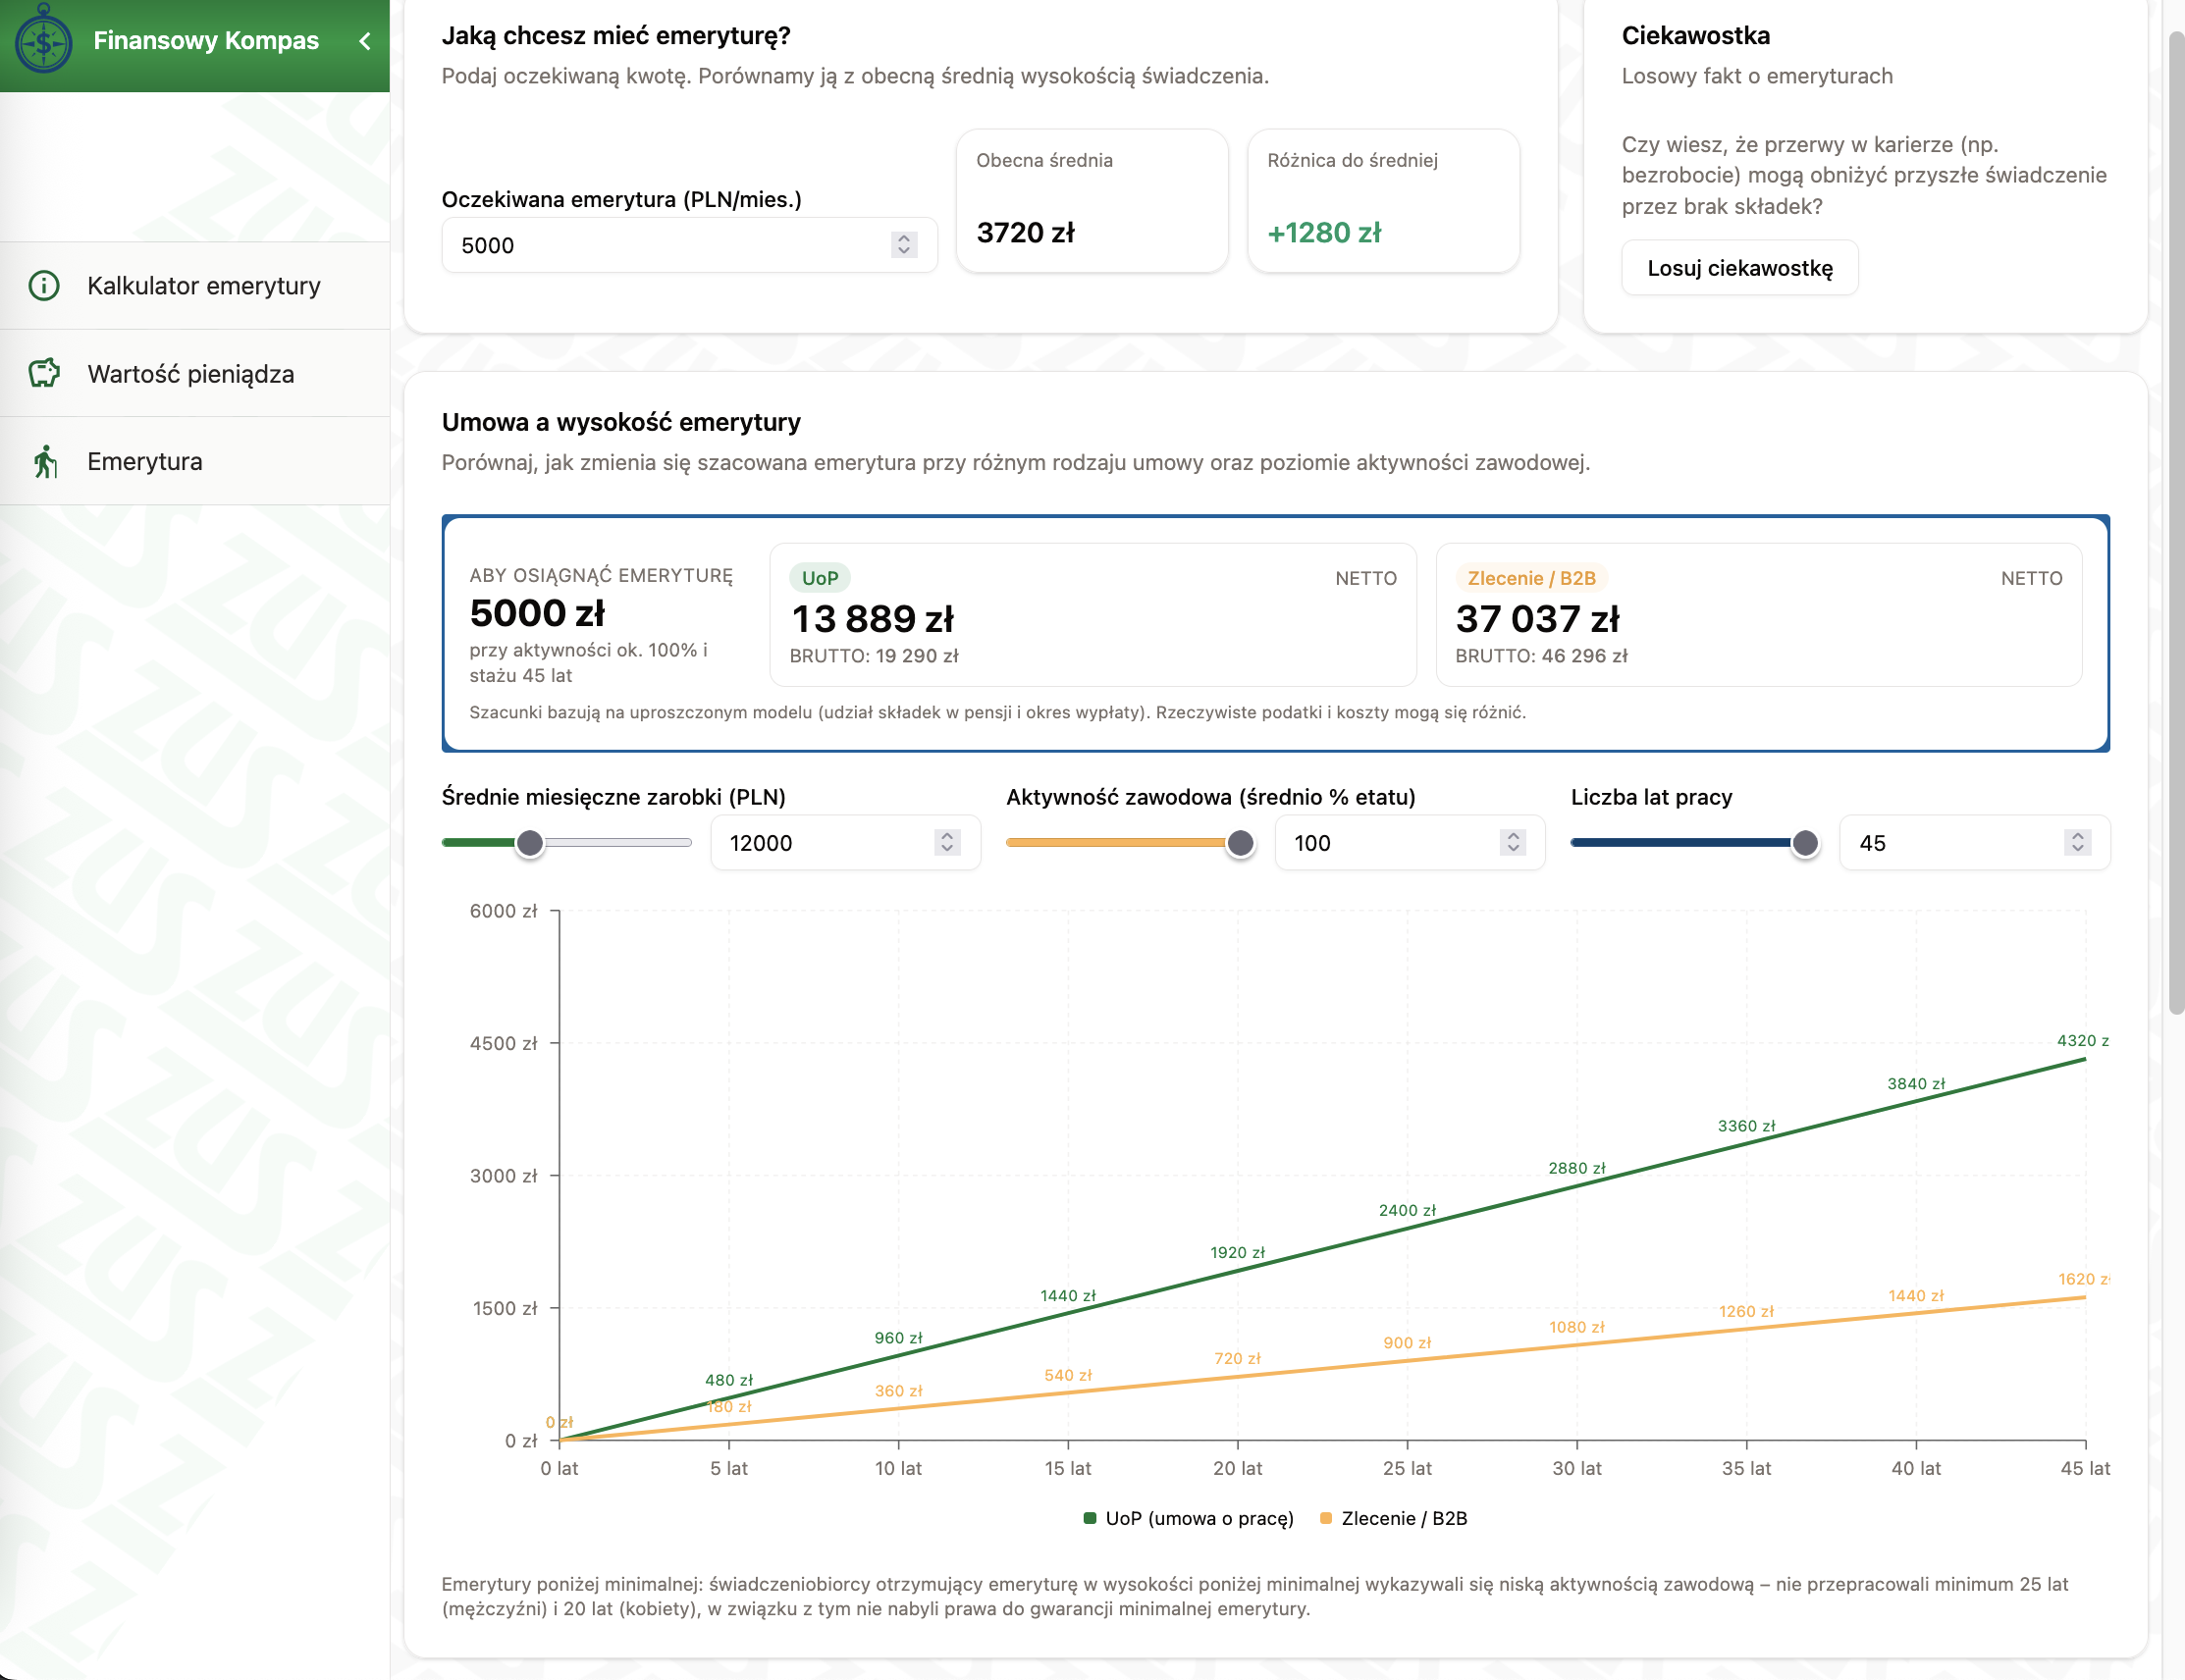
\includegraphics[width=.8\textwidth]{img/module_2_simple_pension_calculator}
\end{frame}

\begin{frame}[t]{Moduł II}{Uproszczony kalkulator emerytalny}
Dynamiczny wykres ilustrujący zależność między planowaną emeryturą nominalną a historią zatrudnienia:
\begin{itemize}
  \item średnimi zarobkami,
  \item stażem aktywności zawodowej,
  \item wymiarem etatu.
\end{itemize}
\end{frame}

\begin{frame}[t]{Moduł II}{Uproszczony kalkulator emerytalny}
Moduł umożliwia także porównanie emerytury osoby zatrudnionej na umowę o pracę
z osobą prowadzącą jednoosobową działalność gospodarczą (B2B),
przy założeniu minimalnego, zgodnego z przepisami, wkładu do ZUS.
\end{frame}

\begin{frame}[t]{Moduł II}{Uproszczony kalkulator emerytalny}
Moduł prezentuje również kontekstowe ciekawostki —
subtelnie edukujące młodych użytkowników o kluczowych elementach systemu emerytalnego.
\end{frame}

\begin{frame}[t]{Moduł II}{Uproszczony kalkulator emerytalny}
Dodatkowo: wykres prezentujący medianę emerytury dla dziesięciu zawodów
losowo wybranych w momencie załadowania strony.
\\[2em]
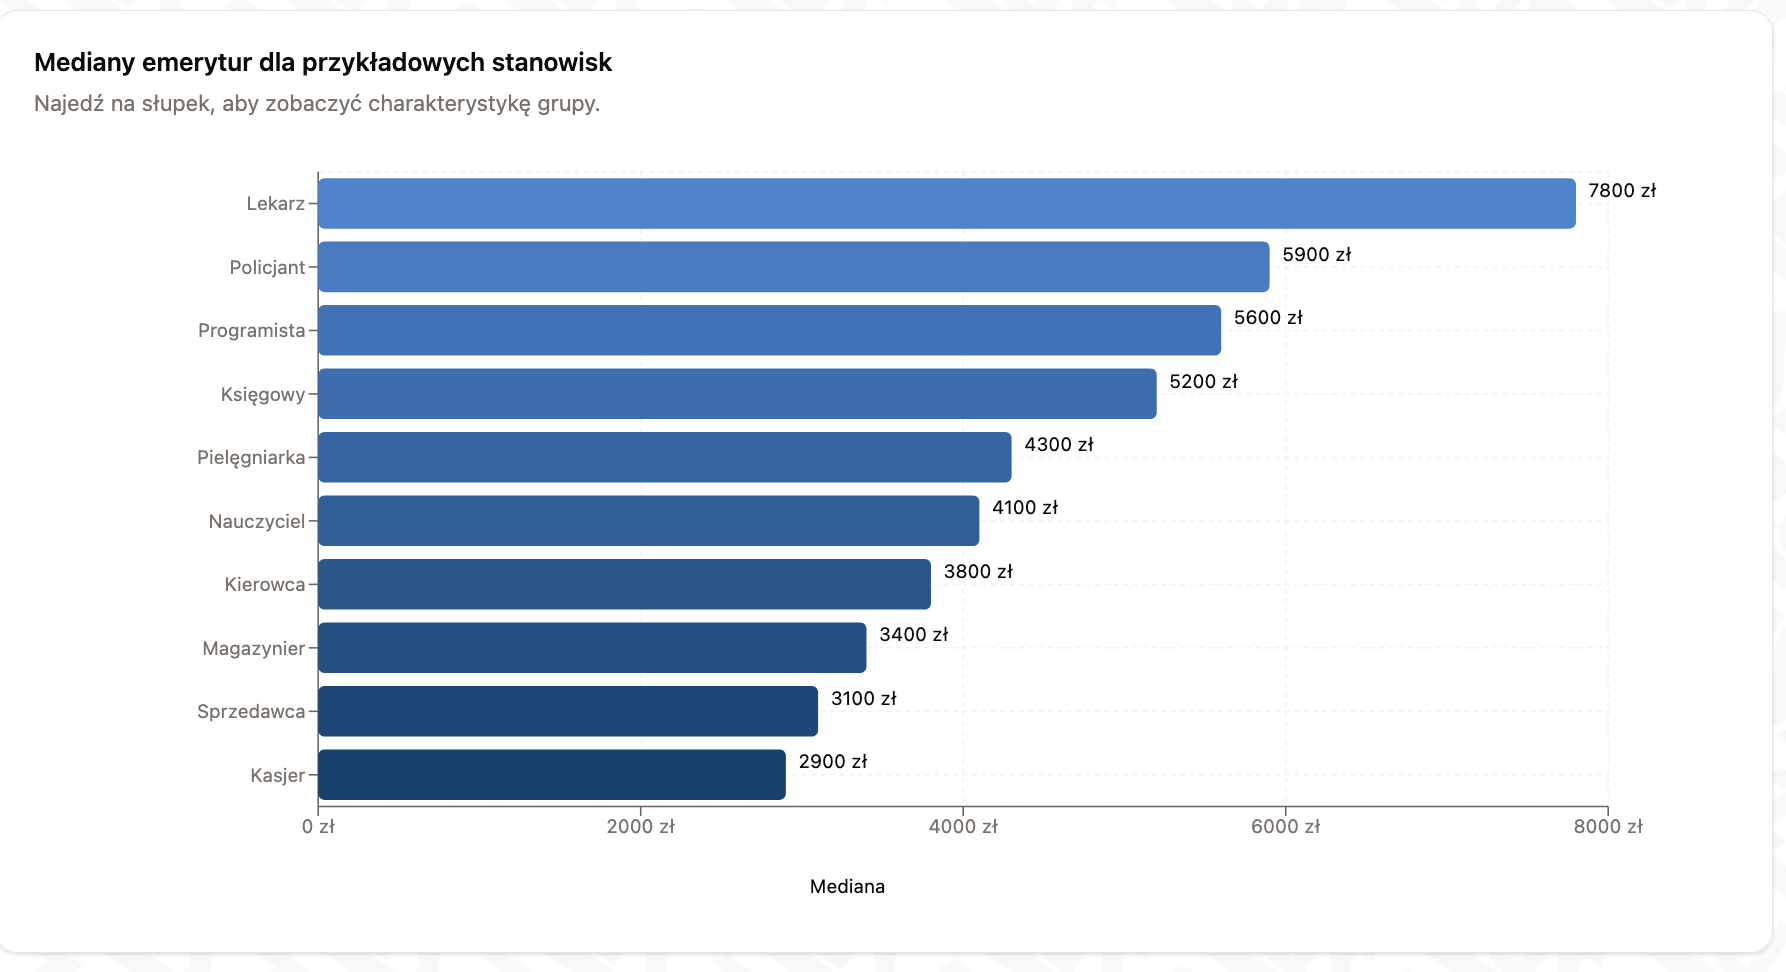
\includegraphics[width=.8\textwidth]{img/module_2b_median_pensions}
\end{frame}

\subsection{Moduł III --- Wartość pieniądza}

\begin{frame}[t]{Moduł III}{Wartość pieniądza}
  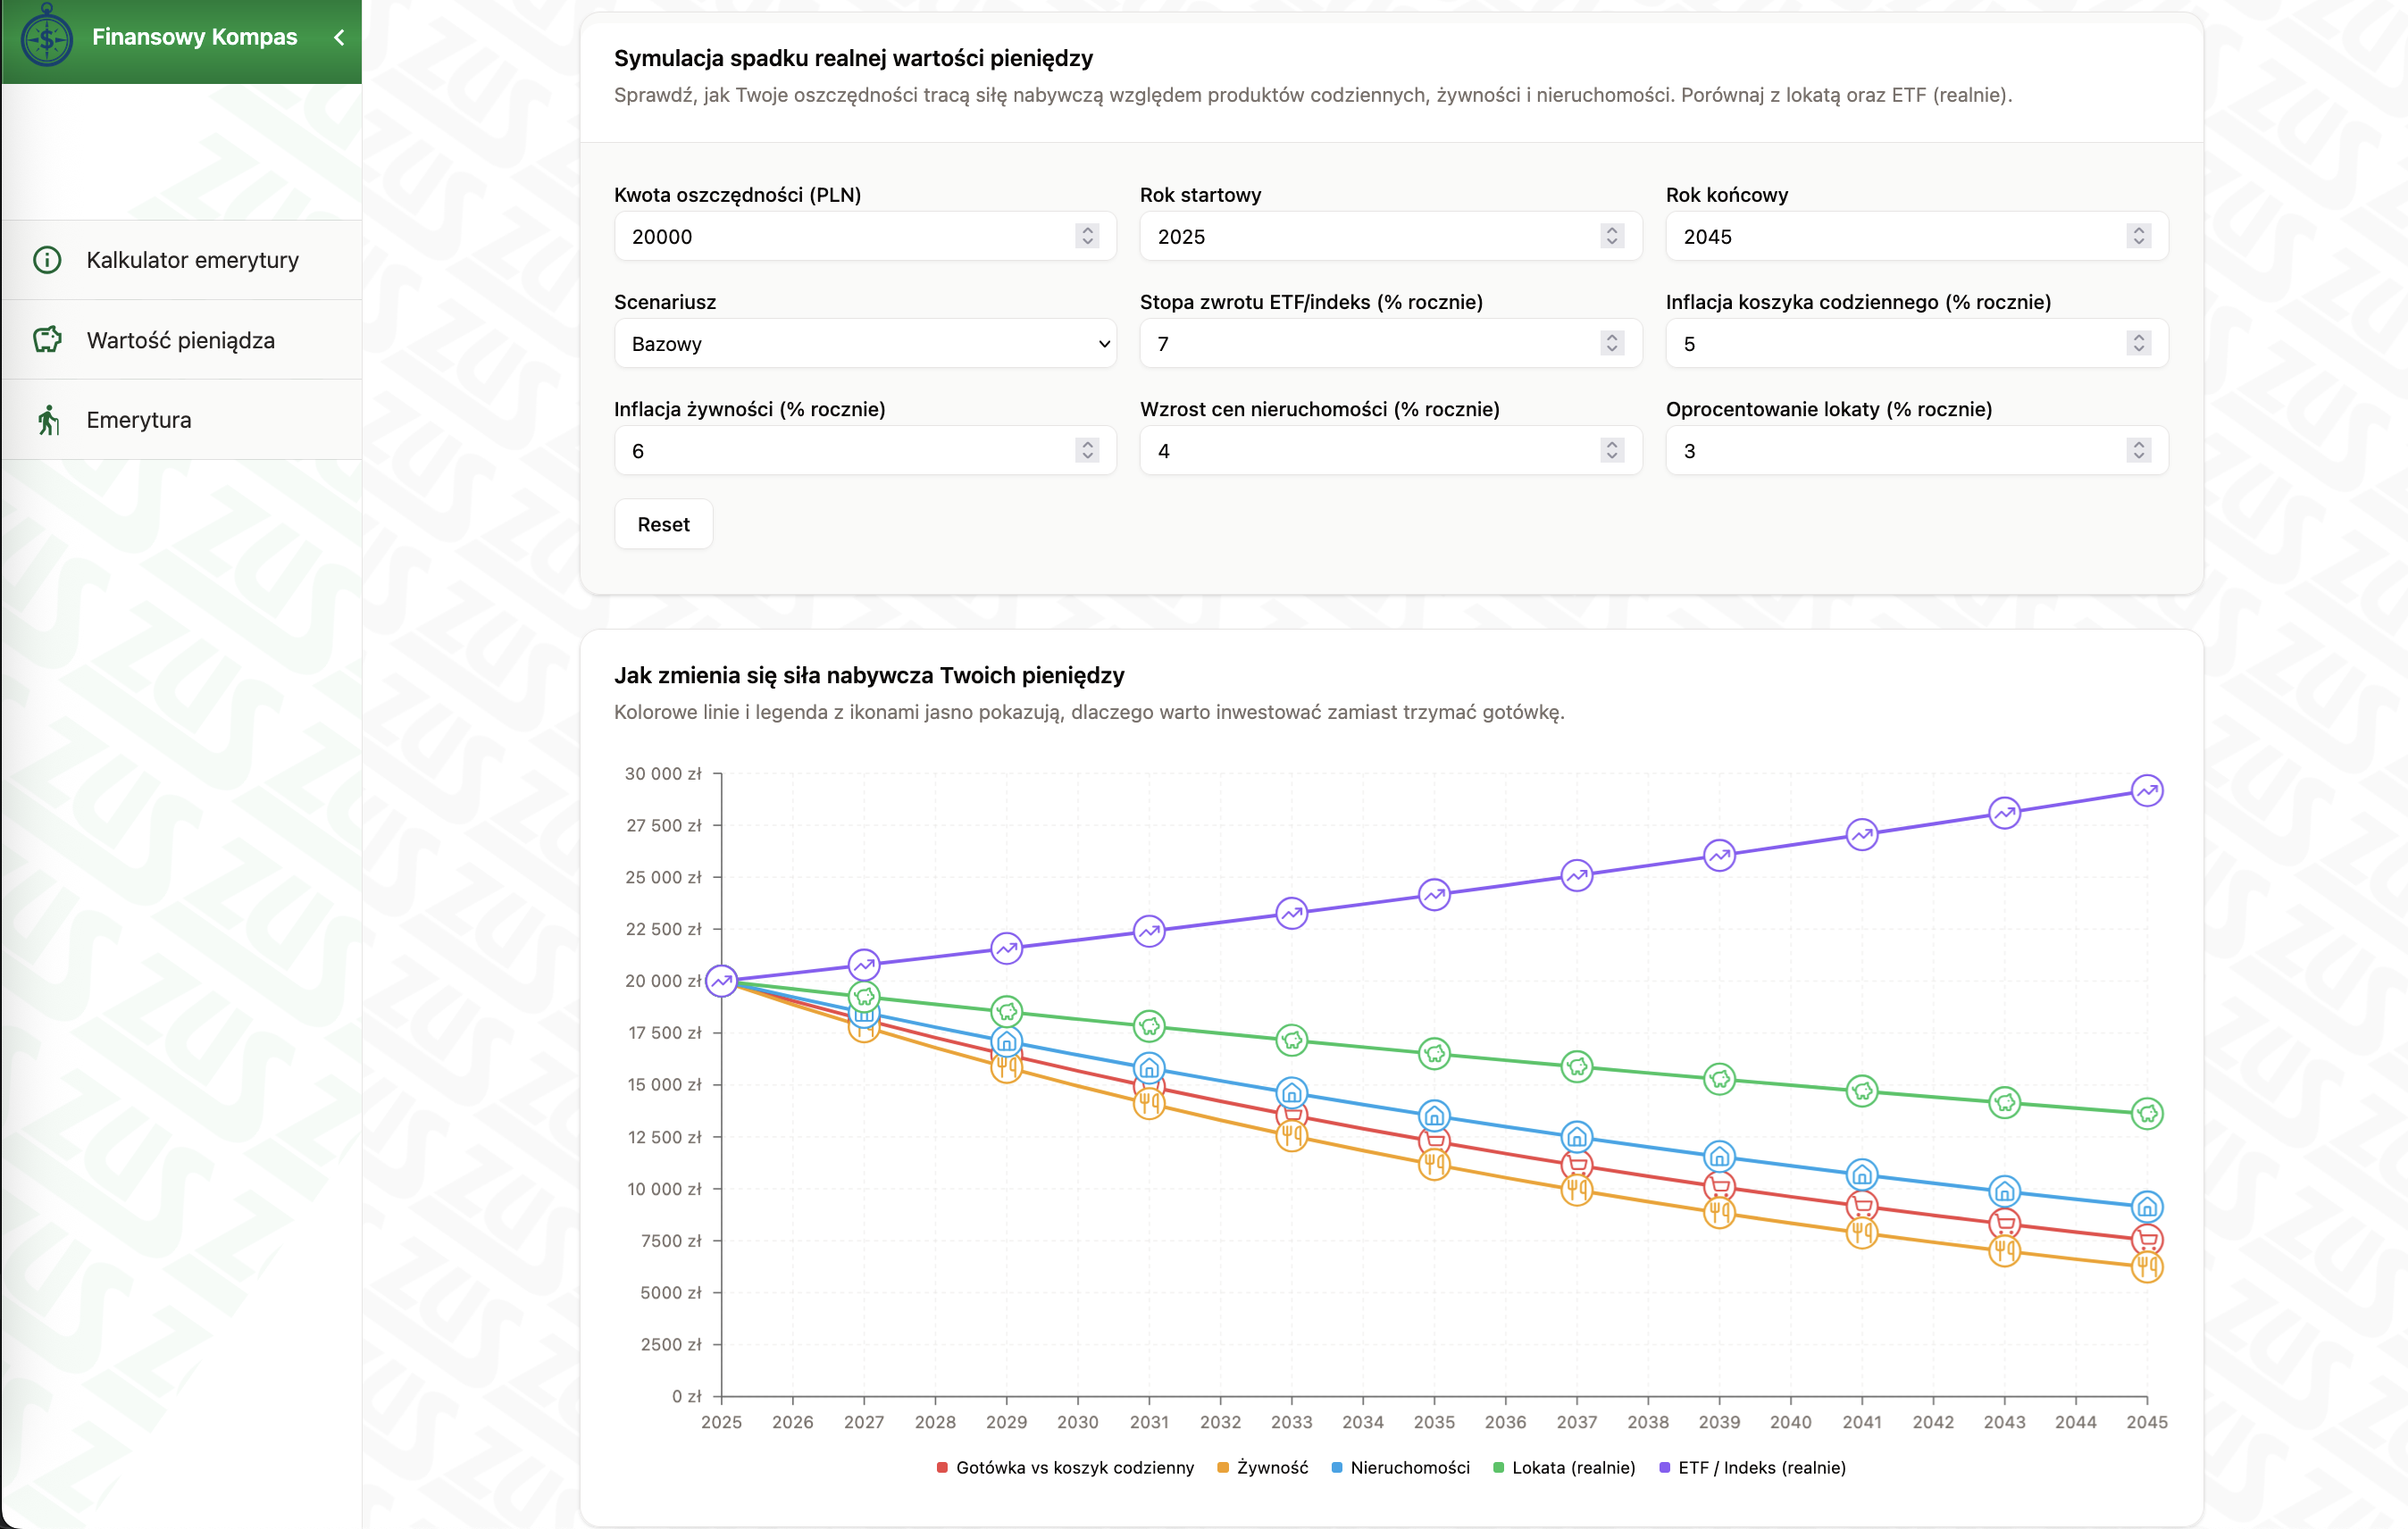
\includegraphics[width=.8\textwidth]{img/module_3_the_value_of_money}
\end{frame}

\begin{frame}[t]{Moduł III}{Wartość pieniądza}
Celem modulu ,,Wartość pieniądza'' jest urealnienie pojęcia inflacji.

\pause
Dzięki konfigurowalnym scenariuszom użytkownik obserwuje na wykresie,
jak zmienia się wartość oszczędności trzymanych na koncie oszczędnościowym lub lokacie.
\pause
Dla porównania uwzględniamy także: rosnące ceny żywności i nieruchomości
oraz dane dotyczące globalnych akcji (zdywersyfikowany fundusz ETF).


\pause Dla porównania wykres zawiera też dane
na temat rosnących cen podstawowych dóbr materialnych: żywności, nieruchomości
oraz przykładowe dane globalnych akcji w formie zdywersyfikowanego funduszu ETF.
\end{frame}

\subsection{Moduł IV --- Rozszerzony kalkulator emerytalny}

\begin{frame}[t]{Moduł IV}{Rozszerzony kalkulator emerytalny}
  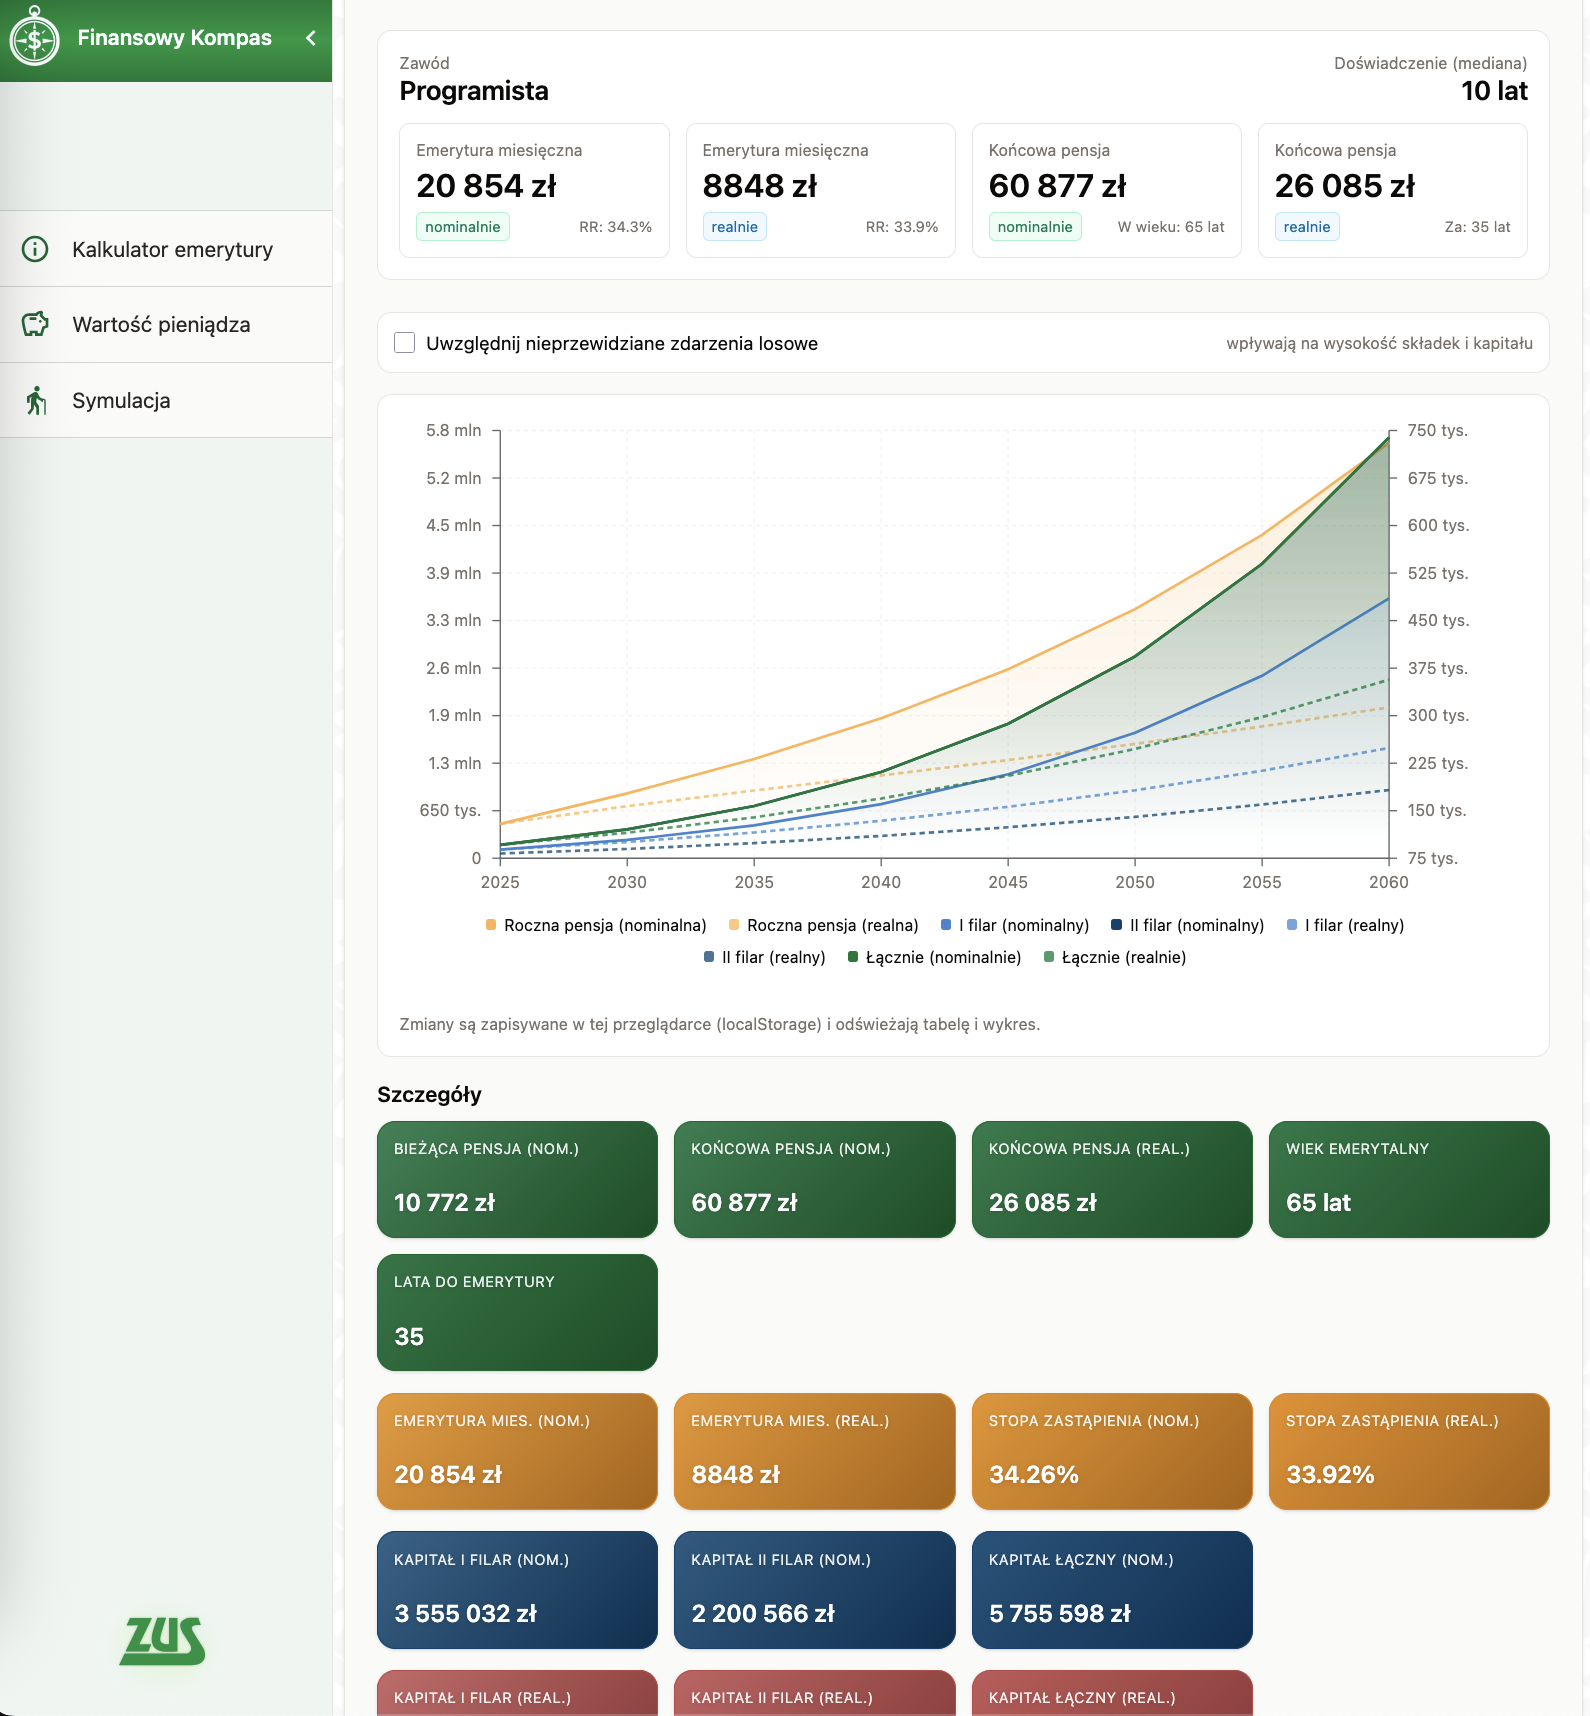
\includegraphics[width=.8\textwidth]{img/module_4_extended_pension_calculator}
\end{frame}

\begin{frame}[t]{Moduł IV}{Rozszerzony kalkulator emerytalny}
Wykorzystujemy pełnię danych od użytkownika (wprowadzonych ręcznie lub wyliczonych z modeli i wartości domyślnych)
i ilustrujemy kluczowe parametry:
\begin{itemize}
  \pause
  \item środki gromadzone na koncie i subkoncie ZUS do końca aktywności zawodowej,
  \pause
  \item ścieżkę zarobków, prognozowaną wartość emerytury oraz stopę zastąpienia ---
        realną, procentową zmianę przychodów w momencie przejścia na emeryturę.
\end{itemize}
\end{frame}

\begin{frame}[t]{Moduł IV}{Rozszerzony kalkulator emerytalny}
W odróżnieniu od modułu II, moduł IV nie tylko wykorzystuje pełnię danych od użytkownika
(wpisanych ręcznie lub wyliczonych z naszych modeli i rozsądnych wartości domyślnych),
ale również ilustruje wszystkie ważne parametry emerytury:

\begin{itemize}
    \pause
    \item wykres, obrazujący pieniądze gromadzone na koncie i subkoncie ZUS przez pozostałe lata aktywności
    zawodowej
    \pause
    \item progresję zarobków, wartości emerytury i tzw. stopę zastąpienia --- realną procentową zmianę
    przychodzu, jakiej nasz użytkownik dozna w momencie przejścia na emeryturę.
\end{itemize}
\end{frame}

\subsection{Moduł V --- Symulacja zdarzeń losowych}

\begin{frame}[t]{Moduł V}{Symulacja zdarzeń losowych}
  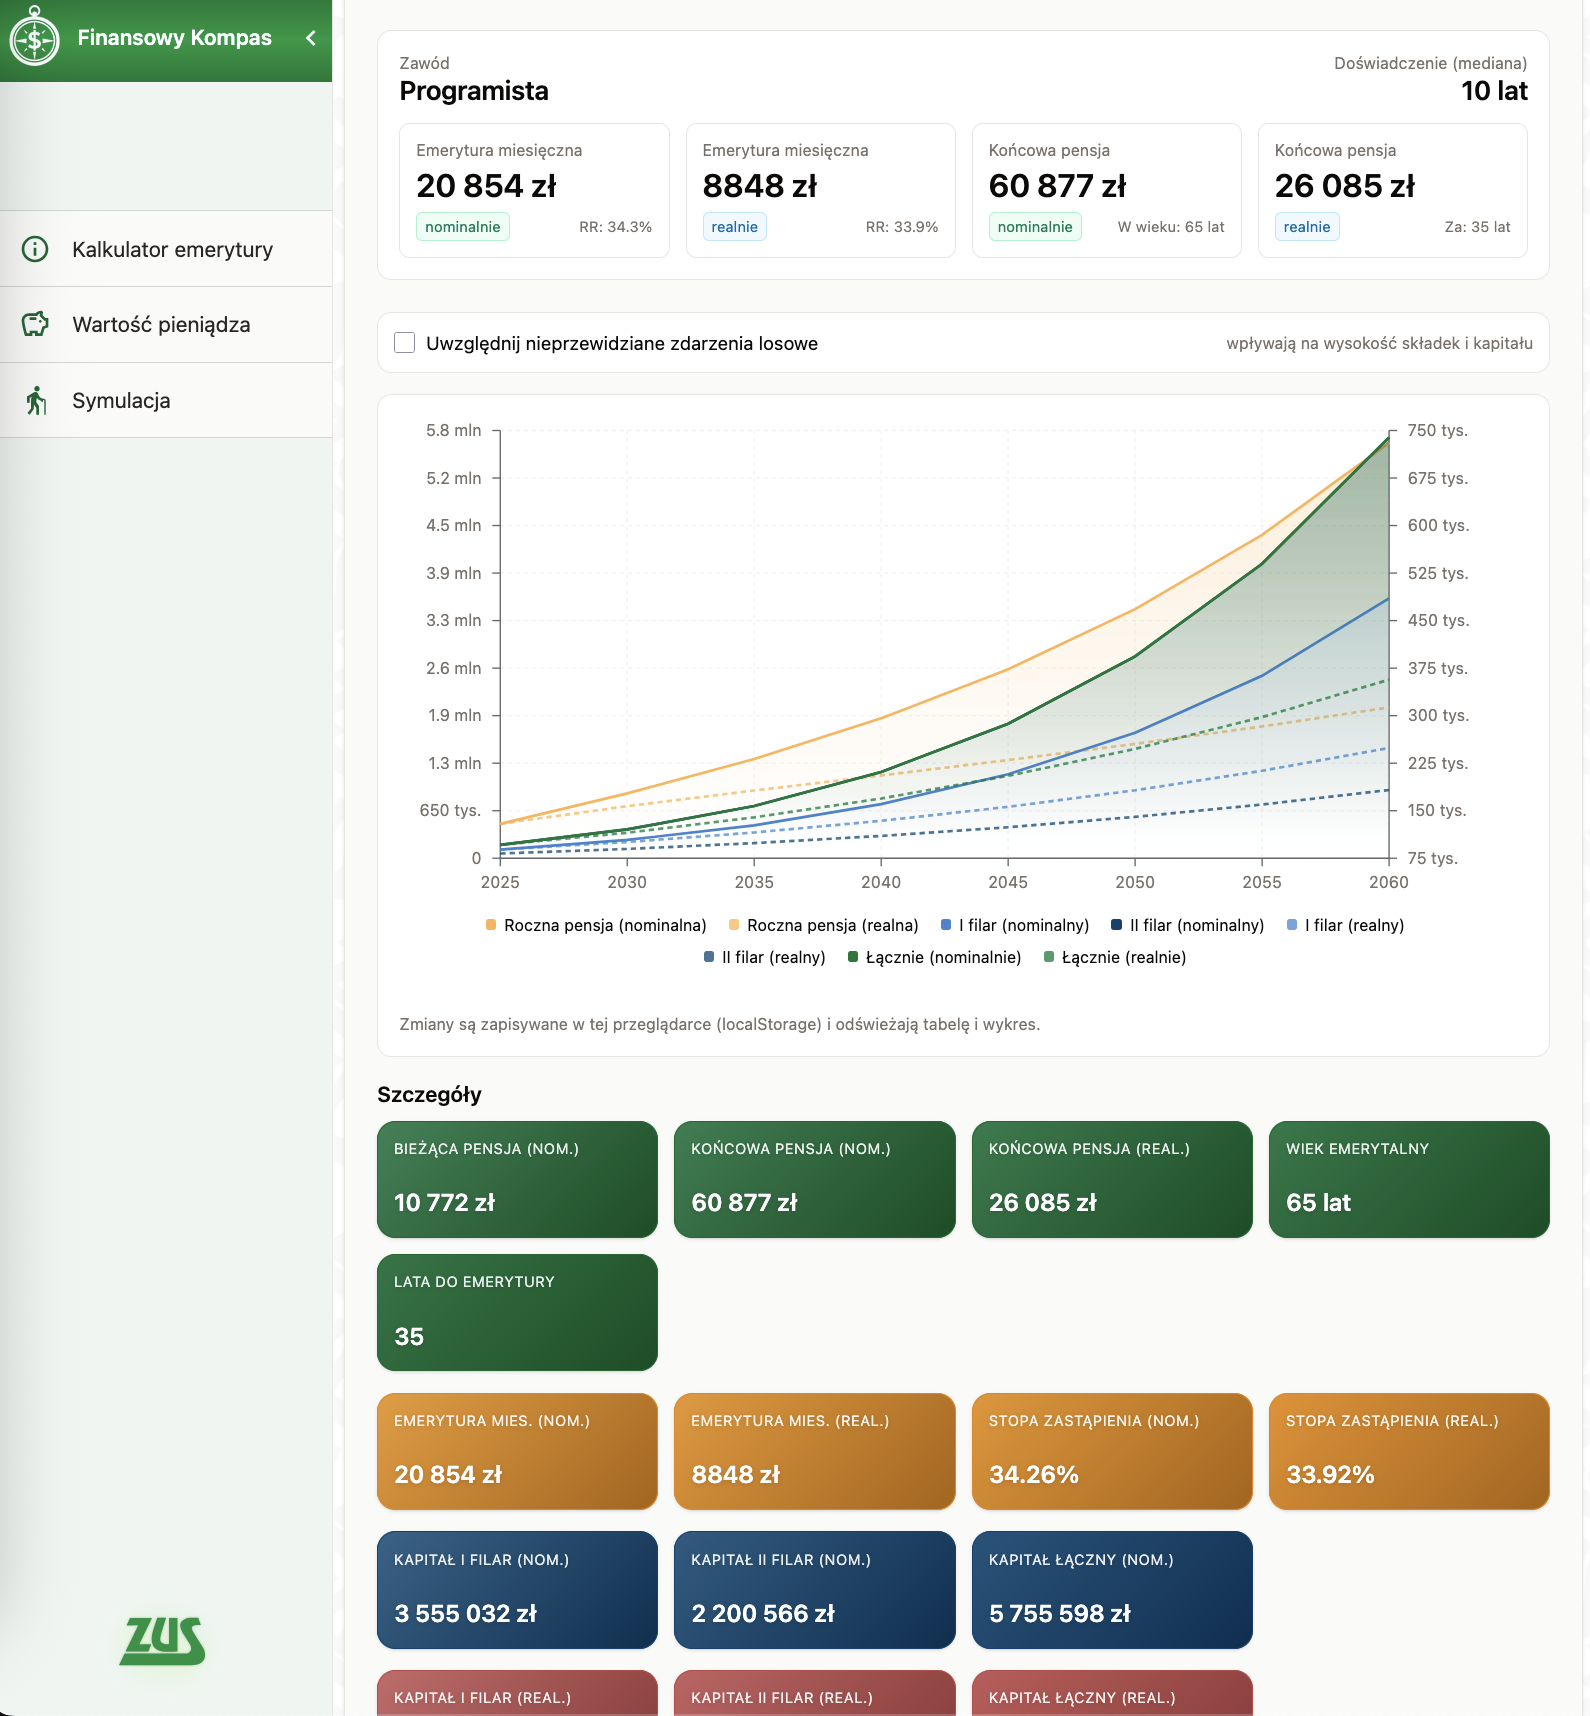
\includegraphics[width=.8\textwidth]{img/module_4_extended_pension_calculator}
\end{frame}

\begin{frame}[t]{Moduł V}{Symulacja zdarzeń losowych}
Opcjonalny moduł, który uwzględnia zdarzenia losowe (utrata pracy, choroba, urlop macierzyński itp.)
w wyliczeniach modułu IV.
\pause
Pozwala zrozumieć, jak silnie wczesne przerwy w zatrudnieniu i odprowadzaniu składek
mogą wpływać na końcową wysokość emerytury.
\end{frame}

\subsection{Moduł VI --- Zbieranie danych statystycznych i generowanie raportu .xls}

\begin{frame}[t]{Moduł VI}{Zbieranie danych statystycznych i generowanie raportu}
Na etapie hackathonu nie wprowadzaliśmy autoryzacji i bazy danych,
jednak zaimplementowaliśmy moduł zbierania anonimowych statystyk,
dostępnych w formie raportu w formacie Excel (.xlsx) dla administratora strony,
zgodnie z wymaganiami zadania.
\end{frame}